\section{CART and Random Forest (RF)}

\subsection{Introduction}

When we model a response variable $Y$ based on one or more predictors $X_1, X_2,\break ..., X_p$, we are solving either a:
\begin{itemize}
    \item \textbf{Regression problem}: $Y$ is \hl{numeric} (quantitative). For example, predicting test scores, house prices, salaries. The \emph{goal} is \textbf{estimate a continuous value}.
    \item \textbf{Classification problem}: $Y$ is \hl{categorical} (qualitative). For example, predicting whether an email is spam or not, or diagnosing a disease type. The \emph{goal} is \textbf{assign each input to one of a finite set of classes} (e.g., ``yes'' or ``no'', or 5 cancer types).
\end{itemize}
Formally, we observe:
\begin{equation*}
    \left(\mathbf{x}_1, y_1\right), \; \left(\mathbf{x}_2, y_2\right), \; \dots, \; \left(\mathbf{x}_n, y_n\right)
    \quad
    \text{with } \mathbf{x}_i = \left(x_{i1}, x_{i2}, \dots, x_{ip}\right)
\end{equation*}
And aim to predict $y_{n+1}$ given a new observation $\mathbf{x}_{n+1}$.

\highspace
\begin{flushleft}
    \textcolor{Green3}{\faIcon{question-circle} \textbf{Motivation for Using Decision Tree}}
\end{flushleft}
Tree-based methods are powerful alternatives to linear models because:
\begin{itemize}[label=\textcolor{Green3}{\faIcon{check}}]
    \item They \textbf{relax parametric assumptions} (e.g., no need to assume linearity or normality).
    \item They \textbf{automatically model variable interactions}, which can be hard to include explicitly in a linear model.
    \item They produce \textbf{interpretable models} with clear decision rules.
\end{itemize}
Tree methods split the input space into simple \textbf{rectangular regions}, where predictions are made by:
\begin{itemize}
    \item \textbf{Mean} of $y$ in the region (regression).
    \item \textbf{Mode} (most frequent class) in the region (classification).
\end{itemize}
This structure is visual and intuitive:
\begin{center}
    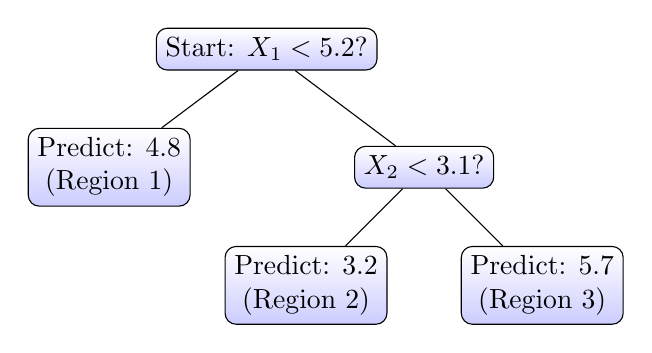
\begin{tikzpicture}[
        level 1/.style={sibling distance=40mm},
        level 2/.style={sibling distance=30mm},
        every node/.style={shape=rectangle, rounded corners, draw, align=center, top color=white, bottom color=blue!20}
    ]

        \node {Start: $X_1 < 5.2$?}
        child {
            node {Predict: 4.8\\(Region 1)}
        }
        child {
            node {$X_2 < 3.1$?}
            child {
                node {Predict: 3.2\\(Region 2)}
            }
            child {
                node {Predict: 5.7\\(Region 3)}
            }
        };

    \end{tikzpicture}
\end{center}

\newpage

\begin{flushleft}
    \textcolor{Red2}{\faIcon{exclamation-triangle} \textbf{Weaknesses of Linear Models (Motivation for Trees)}}
\end{flushleft}
Linear models (like OLS regression or logistic regression) often fall short due to:
\begin{enumerate}
    \item \important{Parametric assumptions}. Require specific functional form:
    \begin{equation*}
        Y = \beta_0 + \beta_1 X_1 + \cdots + \beta_p X_p + \varepsilon
    \end{equation*}
    Assumptions on linearity, normality, and homoscedasticity may not hold in real data.
    \item \important{Lack of interaction modeling}. Unless manually added (e.g., $X_1 \cdot X_2$), interactions are missed. In contrast, trees \textbf{automatically capture interactions} via sequential splits.
    \item \important{Poor flexiibility for complex relationships}. Nonlinearities and sharp changes in response are poorly handled unless transformed carefully.
\end{enumerate}


\begin{table}[!htp]
    \centering
    \begin{adjustbox}{width={\textwidth},totalheight={\textheight},keepaspectratio}
        \begin{tabular}{@{} l l l @{}}
            \toprule
            \textbf{Feature} & \textbf{Linear Models} & \textbf{Decision Trees} \\
            \midrule
            Assumptions                 & Strong                      & Weak                    \\ [.5em]
            Interaction modeling        & Manual                      & Automatic               \\ [.5em]
            Interpretability            & Moderate                    & High (rules, tree)      \\ [.5em]
            Handling nonlinear patterns & Limited                     & Good                    \\ [.5em]
            Overfitting risk            & Lower (with regularization) & Higher (pruning needed) \\
            \bottomrule
        \end{tabular}
    \end{adjustbox}
\end{table}